\subsection{Benchmark}
Student clearly defines a benchmark result or threshold for comparing performances of solutions obtained.

For the CNNs architecture, it is quite important to decide the number of layers.Therefore, I first choose several convolutional layers and decide one of them as a benchmark.

When deciding the architecture, I set the mutual parameters as follows.
The number of batch size is 32.The number of filters of each convolutional layer is 32. and finally the number of epochs is 20.

I tried 4 architecture of CNNs.

\begin{enumerate}
 \item 1 Convolutional layer  2 Fully connected layers \\
 The simplest version in these model.The input and output dimension on each layer are below.
 The accuracy rate of training and validation data are also below.
 
 \begin{figure}[htbp]

	\begin{center}
	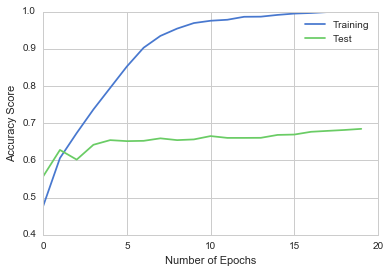
\includegraphics[width=5cm]{picture/1layer_cnn.png}
	\caption{Accuracy rate of training and validation data}
	\end{center}
	\label{fig:eight}

\end{figure}
 
 \item 2 Convolutional layers  2 Fully connected layers \\
 The input and output dimension on each layer are below.
 The accuracy rate of training and validation data are also below.
 
 \begin{figure}[htbp]

	\begin{center}
	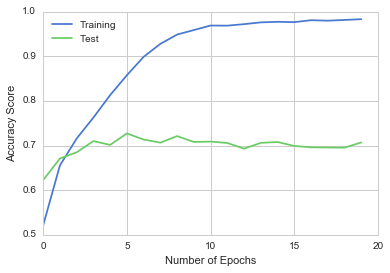
\includegraphics[width=5cm]{picture/2layer_cnn.png}
	\caption{Accuracy rate of training and validation data}
	\end{center}
	\label{fig:nine}

\end{figure}


 \item 3 Convolutional layers 2 Fully connected layers \\
 The accuracy rate of training and validation data are also below.
 
 \begin{figure}[htbp]

	\begin{center}
	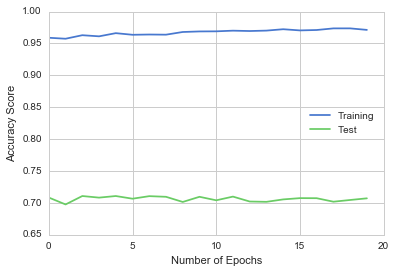
\includegraphics[width=5cm]{picture/3layer_cnn.png}
	\caption{Accuracy rate of training and validation data}
	\end{center}
	\label{fig:ten}

\end{figure}
 \item 4 Convolutional layers 2 Fully connected layers \\
 The accuracy rate of training and validation data are also below.
 
 \begin{figure}[htbp]

	\begin{center}
	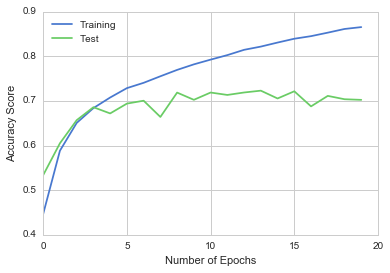
\includegraphics[width=5cm]{picture/4layer_cnn.png}
	\caption{Accuracy rate of training and validation data}
	\end{center}
	\label{fig:eleven}

\end{figure}
\end{enumerate}


From these results, I choose --------- as the benchmark for this task.
